\subsection{getDocumentsByHostnameDomain}
Request Type: \textbf{POST}
\newline
Request Address: \textbf{/getdocumentsbyhostnamedomain}
\newline

This endpoint takes in a JSON document containing a defined hostname and domain with which to query all existing documents that contain the defined hostname and domain in their "run\_information" field, if it exists. The returned data will also be a JSON document that contains all \textbf{unique} documents found in the database, but separated into different documents based on core counts.

It should be noted that only the documents uploaded using the Adapt uploader script found in ParFlow Performance Testing will have the "run\_information" embedded document field, so this will not return any document information taken from data uploaded using Shweta's uploader script.

\subsubsection{Data Format}
\textbf{Required Data}:
\newline
\newline
This endpoint takes in a JSON document in the request body using the format found in Figure \ref{fig:getdocumentsbyhostnamedomain1}. The "String" fields should be replaced with the hostname and domain being used to query. It should be noted that "runname" was the previous key used to define the domain used and the "String" field following "runname" should be the domain.
\begin{figure}[H]
    \centering
    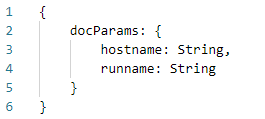
\includegraphics{img/getdocumentsbyhostnamedomain1.PNG}
    \caption{getDocumentsByHostnameDomain Received Data Format}
    \label{fig:getdocumentsbyhostnamedomain1}
\end{figure}
\textbf{Returned Data}:
\newline
\newline
This endpoint will return a JSON document that contains all unique MongoDB documents queried by the hostname and domain, but will split them up based on their core count to ease use in the react app. The API will generate keys in the top level document based off all unique core counts found among the documents. These keys will each have a value containing an embedded document that will hold all MongoDB documents that have a core count matching those keys. These documents are labeled using their provided MongoDB \_id as a key and the value being the raw document data. An example of what this JSON document looks like can be found in Figure \ref{fig:getdocumentsbyhostnamedomain2}.

\begin{figure}[H]
    \centering
    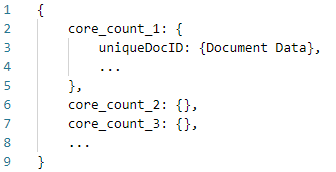
\includegraphics{img/getdocumentsbyhostnamedomain2.PNG}
    \caption{getDocumentsByHostnameDomain Returned Data Format}
    \label{fig:getdocumentsbyhostnamedomain2}
\end{figure}
